
%% bare_adv.tex
%% V1.3
%% 2007/01/11
%% by Michael Shell
%% See: 
%% http://www.michaelshell.org/
%% for current contact information.
%%
%% This is a skeleton file demonstrating the advanced use of IEEEtran.cls
%% (requires IEEEtran.cls version 1.7 or later) with an IEEE Computer
%% Society journal paper.
%%
%% Support sites:
%% http://www.michaelshell.org/tex/ieeetran/
%% http://www.ctan.org/tex-archive/macros/latex/contrib/IEEEtran/
%% and
%% http://www.ieee.org/

%%*************************************************************************
%% Legal Notice:
%% This code is offered as-is without any warranty either expressed or
%% implied; without even the implied warranty of MERCHANTABILITY or
%% FITNESS FOR A PARTICULAR PURPOSE! 
%% User assumes all risk.
%% In no event shall IEEE or any contributor to this code be liable for
%% any damages or losses, including, but not limited to, incidental,
%% consequential, or any other damages, resulting from the use or misuse
%% of any information contained here.
%%
%% All comments are the opinions of their respective authors and are not
%% necessarily endorsed by the IEEE.
%%
%% This work is distributed under the LaTeX Project Public License (LPPL)
%% ( http://www.latex-project.org/ ) version 1.3, and may be freely used,
%% distributed and modified. A copy of the LPPL, version 1.3, is included
%% in the base LaTeX documentation of all distributions of LaTeX released
%% 2003/12/01 or later.
%% Retain all contribution notices and credits.
%% ** Modified files should be clearly indicated as such, including  **
%% ** renaming them and changing author support contact information. **
%%
%% File list of work: IEEEtran.cls, IEEEtran_HOWTO.pdf, bare_adv.tex,
%%                    bare_conf.tex, bare_jrnl.tex, bare_jrnl_compsoc.tex
%%*************************************************************************

% *** Authors should verify (and, if needed, correct) their LaTeX system  ***
% *** with the testflow diagnostic prior to trusting their LaTeX platform ***
% *** with production work. IEEE's font choices can trigger bugs that do  ***
% *** not appear when using other class files.                            ***
% The testflow support page is at:
% http://www.michaelshell.org/tex/testflow/



% IEEEtran V1.7 and later provides for these CLASSINPUT macros to allow the
% user to reprogram some IEEEtran.cls defaults if needed. These settings
% override the internal defaults of IEEEtran.cls regardless of which class
% options are used. Do not use these unless you have good reason to do so as
% they can result in nonIEEE compliant documents. User beware. ;)
%
%\newcommand{\CLASSINPUTbaselinestretch}{1.0} % baselinestretch
%\newcommand{\CLASSINPUTinnersidemargin}{1in} % inner side margin
%\newcommand{\CLASSINPUToutersidemargin}{1in} % outer side margin
%\newcommand{\CLASSINPUTtoptextmargin}{1in}   % top text margin
%\newcommand{\CLASSINPUTbottomtextmargin}{1in}% bottom text margin



% Note that the a4paper option is mainly intended so that authors in
% countries using A4 can easily print to A4 and see how their papers will
% look in print - the typesetting of the document will not typically be
% affected with changes in paper size (but the bottom and side margins will).
% Use the testflow package mentioned above to verify correct handling of
% both paper sizes by the user's LaTeX system.
%
% Also note that the "draftcls" or "draftclsnofoot", not "draft", option
% should be used if it is desired that the figures are to be displayed in
% draft mode.
%
\documentclass[10pt,journal,a4paper]{IEEEtran}
% If IEEEtran.cls has not been installed into the LaTeX system files,
% manually specify the path to it like:
% \documentclass[10pt,journal,compsoc]{../sty/IEEEtran}


% For Computer Society journals, IEEEtran defaults to the use of 
% Palatino/Palladio as is done in IEEE Computer Society journals.
% To go back to Times Roman, you can use this code:
%\renewcommand{\rmdefault}{ptm}\selectfont





% Some very useful LaTeX packages include:
% (uncomment the ones you want to load)



% *** MISC UTILITY PACKAGES ***
%
%\usepackage{ifpdf}
% Heiko Oberdiek's ifpdf.sty is very useful if you need conditional
% compilation based on whether the output is pdf or dvi.
% usage:
% \ifpdf
%   % pdf code
% \else
%   % dvi code
% \fi
% The latest version of ifpdf.sty can be obtained from:
% http://www.ctan.org/tex-archive/macros/latex/contrib/oberdiek/
% Also, note that IEEEtran.cls V1.7 and later provides a builtin
% \ifCLASSINFOpdf conditional that works the same way.
% When switching from latex to pdflatex and vice-versa, the compiler may
% have to be run twice to clear warning/error messages.






% *** CITATION PACKAGES ***
%
\ifCLASSOPTIONcompsoc
  % IEEE Computer Society needs nocompress option
  % requires cite.sty v4.0 or later (November 2003)
  % \usepackage[nocompress]{cite}
\else
  % normal IEEE
  % \usepackage{cite}
\fi
% cite.sty was written by Donald Arseneau
% V1.6 and later of IEEEtran pre-defines the format of the cite.sty package
% \cite{} output to follow that of IEEE. Loading the cite package will
% result in citation numbers being automatically sorted and properly
% "compressed/ranged". e.g., [1], [9], [2], [7], [5], [6] without using
% cite.sty will become [1], [2], [5]--[7], [9] using cite.sty. cite.sty's
% \cite will automatically add leading space, if needed. Use cite.sty's
% noadjust option (cite.sty V3.8 and later) if you want to turn this off.
% cite.sty is already installed on most LaTeX systems. Be sure and use
% version 4.0 (2003-05-27) and later if using hyperref.sty. cite.sty does
% not currently provide for hyperlinked citations.
% The latest version can be obtained at:
% http://www.ctan.org/tex-archive/macros/latex/contrib/cite/
% The documentation is contained in the cite.sty file itself.
%
% Note that some packages require special options to format as the Computer
% Society requires. In particular, Computer Society  papers do not use
% compressed citation ranges as is done in typical IEEE papers
% (e.g., [1]-[4]). Instead, they list every citation separately in order
% (e.g., [1], [2], [3], [4]). To get the latter we need to load the cite
% package with the nocompress option which is supported by cite.sty v4.0
% and later. Note also the use of a CLASSOPTION conditional provided by
% IEEEtran.cls V1.7 and later.





% *** GRAPHICS RELATED PACKAGES ***
%
\ifCLASSINFOpdf
  % \usepackage[pdftex]{graphicx}
  % declare the path(s) where your graphic files are
  % \graphicspath{{../pdf/}{../jpeg/}}
  % and their extensions so you won't have to specify these with
  % every instance of \includegraphics
  % \DeclareGraphicsExtensions{.pdf,.jpeg,.png}
\else
  % or other class option (dvipsone, dvipdf, if not using dvips). graphicx
  % will default to the driver specified in the system graphics.cfg if no
  % driver is specified.
  % \usepackage[dvips]{graphicx}
  % declare the path(s) where your graphic files are
  % \graphicspath{{../eps/}}
  % and their extensions so you won't have to specify these with
  % every instance of \includegraphics
  % \DeclareGraphicsExtensions{.eps}
\fi
% graphicx was written by David Carlisle and Sebastian Rahtz. It is
% required if you want graphics, photos, etc. graphicx.sty is already
% installed on most LaTeX systems. The latest version and documentation can
% be obtained at: 
% http://www.ctan.org/tex-archive/macros/latex/required/graphics/
% Another good source of documentation is "Using Imported Graphics in
% LaTeX2e" by Keith Reckdahl which can be found as epslatex.ps or
% epslatex.pdf at: http://www.ctan.org/tex-archive/info/
%
% latex, and pdflatex in dvi mode, support graphics in encapsulated
% postscript (.eps) format. pdflatex in pdf mode supports graphics
% in .pdf, .jpeg, .png and .mps (metapost) formats. Users should ensure
% that all non-photo figures use a vector format (.eps, .pdf, .mps) and
% not a bitmapped formats (.jpeg, .png). IEEE frowns on bitmapped formats
% which can result in "jaggedy"/blurry rendering of lines and letters as
% well as large increases in file sizes.
%
% You can find documentation about the pdfTeX application at:
% http://www.tug.org/applications/pdftex



%\usepackage{ps4pdf}
% dvi->ps workflow is required to use such packages as psfrag.sty and
% pstricks.sty. However, Rolf Niepraschk's ps4pdf.sty provides a way to
% apply psfrag/pstricks effects to .eps figures and then get the resultant
% figures in .pdf form. Thus, providing an easier way for migrating from
% .eps to .pdf figures. After ps4pdf.sty loads, if:
% 1. producing .dvi output: the output file will consist ONLY of the
%    figures (or other constructs encased within \PSforPDF commands)
% 2. producing .pdf output: pdflatex will look in the filename-pics.pdf
%    file, where filename is the basename of the tex document, for the
%    graphics (or other constructs encased within \PSforPDF commands).
%    NOTE: If you ever change your figures, you must remember to remake
%    the filename-pics.pdf file.
%
% This way you can do a:
% 
% latex filename
% dvips -Ppdf -o filename-pics.ps filename.dvi
% ps2pdf filename-pics.ps filename-pics.pdf
% 
% to produce a filename-pics.pdf graphics container that contains
% .pdf versions of the graphics with psfrag, pstricks, etc. features.
% Note that you will not typically be able to view the figures in 
% filename-pics.ps because of an offset. However, you will be able to
% view them in filename-pics.pdf. Also, note that when ps4pdf is in effect
% with .dvi output, you may get harmless over/under full box warnings - 
% ignore them. 
% Then, run pdflatex:
% 
% pdflatex filename
% 
% to use pdflatex to make PDF output, automatically using the figures in
% filename-pics.pdf. Alternatively, you could use dvips -i option to
% obtain separate .pdf files for each figure:
%
% dvips -Ppdf -i -E -o fig filename
%
% then convert each figure to pdf via a command such as epstopdf and then
% use pdflatex with these pdf figures and then to dispense with ps4pdf.
%
% Remember to rerun through latex/dvips/ps2pdf if you ever change your
% figures so that filename-pics.pdf gets updated.
% ps4pdf requires David Kastrup's preview-latex and a recent LaTeX system
% (circa 2001 or later). The ps4pdf package and documentation can be
% obtained at: http://www.ctan.org/tex-archive/macros/latex/contrib/ps4pdf/
% The preview-latex package and documentation can be obtained at:
% http://www.ctan.org/tex-archive/macros/latex/contrib/preview/
%
% provide a bogus \PSforPDF, even when not loading pd4pdf. This way we can
% stop loading ps4pdf.sty if we choose to make separate .pdf versions of
% each of our figures.
\providecommand{\PSforPDF}[1]{#1}
% Note that in order for ps4pdf to work, all commands related to psfrag,
% pstricks, etc. must be called within the PSforPDF command. This applies
% even when *loading* via \usepackage psfrag.sty, etc.


%\PSforPDF{\usepackage{psfrag}}
% psfrag.sty was written by Craig Barratt, Michael C. Grant, and
% David Carlisle. It allows you to substitute LaTeX commands for text in
% imported EPS graphic files. In this way, LaTeX symbols can be placed into
% graphics that have been generated by other applications. You must use
% latex->dvips->ps2pdf workflow (not direct pdf output from pdflatex) if
% you wish to use this capability because it works via some PostScript
% tricks. Alternatively, the graphics could be processed as separate files
% via psfrag and dvips, then converted to PDF for inclusion in the main file
% which uses pdflatex. ps4pdf.sty (above) provides a way of doing this all
% at once within the main file.
% Docs are in "The PSfrag System" by Michael C. Grant and David Carlisle.
% There is also some information about using psfrag in "Using Imported
% Graphics in LaTeX2e" by Keith Reckdahl which documents the graphicx
% package (see above). The psfrag package and documentation can be obtained
% at: http://www.ctan.org/tex-archive/macros/latex/contrib/psfrag/
% 
% Note that the current version of psfrag does not "turn itself off" when
% running under pdf output. This will result in a harmless warning
% about a non-PDF \special. However, to silence this, a bogus psfrag
% command can be provided instead of loading psfrag.sty when PDF output
% is being used. Thus, a more complex alternative conditional loading scheme
% can be employed instead of the straightforword way above:
%
%\ifCLASSINFOpdf
% if outputting PDF, do not use or load psfrag.sty as current versions
% output a non-PDF special that generates a harmless, but annoying warning.
% Instead, we provide a bogus \psfrag command that does nothing with
% its arguments. This is a tad tricky because \psfrag can have up to six
% arguments four of which are optional: \psfrag{}[][][][]{}
% Code based on that in psfrag.sty
%\makeatletter
%\def\psfrag{\@ifstar{\@BOGUSpsfraga}{\@BOGUSpsfraga}}
%\def\@BOGUSpsfraga{\begingroup
%   \@makeother\"\@makeother\*\@makeother\!\@makeother\~%
%   \@makeother\:\@makeother\\\@makeother\%\@makeother\#%
%   \@makeother\ \@BOGUSpsfragb}
%\def\@BOGUSpsfragb#1{\endgroup
%                \@ifnextchar [{\@BOGUSpsfragc}%
%                              {\@BOGUSpsfrag}}
%\def\@BOGUSpsfragc[#1]{\@ifnextchar [{\@BOGUSpsfragd}%
%                                     {\@BOGUSpsfrag}}
%\def\@BOGUSpsfragd[#1]{\@ifnextchar [{\@BOGUSpsfrage}%
%                                     {\@BOGUSpsfrag}}
%\def\@BOGUSpsfrage[#1]{\@ifnextchar [{\@BOGUSpsfragf}%
%                                     {\@BOGUSpsfrag}}
%\def\@BOGUSpsfragf[#1]{\@BOGUSpsfrag}
%\def\@BOGUSpsfrag#1{\ignorespaces}
%\makeatother
%\else
% using dvi output, load psfrag, but funnel it through PSforPDF
% as required by ps4pdf.sty
%\PSforPDF{\usepackage{psfrag}}
%\fi





% *** MATH PACKAGES ***
%
\usepackage[cmex10]{amsmath}
% A popular package from the American Mathematical Society that provides
% many useful and powerful commands for dealing with mathematics. If using
% it, be sure to load this package with the cmex10 option to ensure that
% only type 1 fonts will utilized at all point sizes. Without this option,
% it is possible that some math symbols, particularly those within
% footnotes, will be rendered in bitmap form which will result in a
% document that can not be IEEE Xplore compliant!
%
% Also, note that the amsmath package sets \interdisplaylinepenalty to 10000
% thus preventing page breaks from occurring within multiline equations. Use:
%\interdisplaylinepenalty=2500
% after loading amsmath to restore such page breaks as IEEEtran.cls normally
% does. amsmath.sty is already installed on most LaTeX systems. The latest
% version and documentation can be obtained at:
% http://www.ctan.org/tex-archive/macros/latex/required/amslatex/math/





% *** SPECIALIZED LIST PACKAGES ***
%\usepackage{acronym}
% acronym.sty was written by Tobias Oetiker. This package provides tools for
% managing documents with large numbers of acronyms. (You don't *have* to
% use this package - unless you have a lot of acronyms, you may feel that
% such package management of them is bit of an overkill.)
% Do note that the acronym environment (which lists acronyms) will have a
% problem when used under IEEEtran.cls because acronym.sty relies on the
% description list environment - which IEEEtran.cls has customized for
% producing IEEE style lists. A workaround is to declared the longest
% label width via the IEEEtran.cls \IEEEiedlistdecl global control:
%
% \renewcommand{\IEEEiedlistdecl}{\IEEEsetlabelwidth{SONET}}
% \begin{acronym}
%
% \end{acronym}
% \renewcommand{\IEEEiedlistdecl}{\relax}% remember to reset \IEEEiedlistdecl
%
% instead of using the acronym environment's optional argument.
% The latest version and documentation can be obtained at:
% http://www.ctan.org/tex-archive/macros/latex/contrib/acronym/


%\usepackage{algorithmic}
% algorithmic.sty was written by Peter Williams and Rogerio Brito.
% This package provides an algorithmic environment fo describing algorithms.
% You can use the algorithmic environment in-text or within a figure
% environment to provide for a floating algorithm. Do NOT use the algorithm
% floating environment provided by algorithm.sty (by the same authors) or
% algorithm2e.sty (by Christophe Fiorio) as IEEE does not use dedicated
% algorithm float types and packages that provide these will not provide
% correct IEEE style captions. The latest version and documentation of
% algorithmic.sty can be obtained at:
% http://www.ctan.org/tex-archive/macros/latex/contrib/algorithms/
% There is also a support site at:
% http://algorithms.berlios.de/index.html
% Also of interest may be the (relatively newer and more customizable)
% algorithmicx.sty package by Szasz Janos:
% http://www.ctan.org/tex-archive/macros/latex/contrib/algorithmicx/




% *** ALIGNMENT PACKAGES ***
%
%\usepackage{array}
% Frank Mittelbach's and David Carlisle's array.sty patches and improves
% the standard LaTeX2e array and tabular environments to provide better
% appearance and additional user controls. As the default LaTeX2e table
% generation code is lacking to the point of almost being broken with
% respect to the quality of the end results, all users are strongly
% advised to use an enhanced (at the very least that provided by array.sty)
% set of table tools. array.sty is already installed on most systems. The
% latest version and documentation can be obtained at:
% http://www.ctan.org/tex-archive/macros/latex/required/tools/


%\usepackage{mdwmath}
%\usepackage{mdwtab}
% Also highly recommended is Mark Wooding's extremely powerful MDW tools,
% especially mdwmath.sty and mdwtab.sty which are used to format equations
% and tables, respectively. The MDWtools set is already installed on most
% LaTeX systems. The lastest version and documentation is available at:
% http://www.ctan.org/tex-archive/macros/latex/contrib/mdwtools/


% IEEEtran contains the IEEEeqnarray family of commands that can be used to
% generate multiline equations as well as matrices, tables, etc., of high
% quality.


%\usepackage{eqparbox}
% Also of notable interest is Scott Pakin's eqparbox package for creating
% (automatically sized) equal width boxes - aka "natural width parboxes".
% Available at:
% http://www.ctan.org/tex-archive/macros/latex/contrib/eqparbox/





% *** SUBFIGURE PACKAGES ***
%\ifCLASSOPTIONcompsoc
%\usepackage[tight,normalsize,sf,SF]{subfigure}
%\else
%\usepackage[tight,footnotesize]{subfigure}
%\fi
% subfigure.sty was written by Steven Douglas Cochran. This package makes it
% easy to put subfigures in your figures. e.g., "Figure 1a and 1b". For IEEE
% work, it is a good idea to load it with the tight package option to reduce
% the amount of white space around the subfigures. Computer Society papers
% use a larger font and \sffamily font for their captions, hence the
% additional options needed under compsoc mode. subfigure.sty is already
% installed on most LaTeX systems. The latest version and documentation can
% be obtained at:
% http://www.ctan.org/tex-archive/obsolete/macros/latex/contrib/subfigure/
% subfigure.sty has been superceeded by subfig.sty.


%\ifCLASSOPTIONcompsoc
%  \usepackage[caption=false]{caption}
%  \usepackage[font=normalsize,labelfont=sf,textfont=sf]{subfig}
%\else
%  \usepackage[caption=false]{caption}
%  \usepackage[font=footnotesize]{subfig}
%\fi
% subfig.sty, also written by Steven Douglas Cochran, is the modern
% replacement for subfigure.sty. However, subfig.sty requires and
% automatically loads Axel Sommerfeldt's caption.sty which will override
% IEEEtran.cls handling of captions and this will result in nonIEEE style
% figure/table captions. To prevent this problem, be sure and preload
% caption.sty with its "caption=false" package option. This is will preserve
% IEEEtran.cls handing of captions. Version 1.3 (2005/06/28) and later 
% (recommended due to many improvements over 1.2) of subfig.sty supports
% the caption=false option directly:
%\ifCLASSOPTIONcompsoc
%  \usepackage[caption=false,font=normalsize,labelfont=sf,textfont=sf]{subfig}
%\else
%  \usepackage[caption=false,font=footnotesize]{subfig}
%\fi
%
% The latest version and documentation can be obtained at:
% http://www.ctan.org/tex-archive/macros/latex/contrib/subfig/
% The latest version and documentation of caption.sty can be obtained at:
% http://www.ctan.org/tex-archive/macros/latex/contrib/caption/




% *** FLOAT PACKAGES ***
%
%\usepackage{fixltx2e}
% fixltx2e, the successor to the earlier fix2col.sty, was written by
% Frank Mittelbach and David Carlisle. This package corrects a few problems
% in the LaTeX2e kernel, the most notable of which is that in current
% LaTeX2e releases, the ordering of single and double column floats is not
% guaranteed to be preserved. Thus, an unpatched LaTeX2e can allow a
% single column figure to be placed prior to an earlier double column
% figure. The latest version and documentation can be found at:
% http://www.ctan.org/tex-archive/macros/latex/base/


%\usepackage{stfloats}
% stfloats.sty was written by Sigitas Tolusis. This package gives LaTeX2e
% the ability to do double column floats at the bottom of the page as well
% as the top. (e.g., "\begin{figure*}[!b]" is not normally possible in
% LaTeX2e). It also provides a command:
%\fnbelowfloat
% to enable the placement of footnotes below bottom floats (the standard
% LaTeX2e kernel puts them above bottom floats). This is an invasive package
% which rewrites many portions of the LaTeX2e float routines. It may not work
% with other packages that modify the LaTeX2e float routines. The latest
% version and documentation can be obtained at:
% http://www.ctan.org/tex-archive/macros/latex/contrib/sttools/
% Documentation is contained in the stfloats.sty comments as well as in the
% presfull.pdf file. Do not use the stfloats baselinefloat ability as IEEE
% does not allow \baselineskip to stretch. Authors submitting work to the
% IEEE should note that IEEE rarely uses double column equations and
% that authors should try to avoid such use. Do not be tempted to use the
% cuted.sty or midfloat.sty packages (also by Sigitas Tolusis) as IEEE does
% not format its papers in such ways.


%\ifCLASSOPTIONcaptionsoff
%  \usepackage[nomarkers]{endfloat}
% \let\MYoriglatexcaption\caption
% \renewcommand{\caption}[2][\relax]{\MYoriglatexcaption[#2]{#2}}
%\fi
% endfloat.sty was written by James Darrell McCauley and Jeff Goldberg.
% This package may be useful when used in conjunction with IEEEtran.cls'
% captionsoff option. Some IEEE journals/societies require that submissions
% have lists of figures/tables at the end of the paper and that
% figures/tables without any captions are placed on a page by themselves at
% the end of the document. If needed, the draftcls IEEEtran class option or
% \CLASSINPUTbaselinestretch interface can be used to increase the line
% spacing as well. Be sure and use the nomarkers option of endfloat to
% prevent endfloat from "marking" where the figures would have been placed
% in the text. The two hack lines of code above are a slight modification of
% that suggested by in the endfloat docs (section 8.3.1) to ensure that
% the full captions always appear in the list of figures/tables - even if
% the user used the short optional argument of \caption[]{}.
% IEEE papers do not typically make use of \caption[]'s optional argument,
% so this should not be an issue. A similar trick can be used to disable
% captions of packages such as subfig.sty that lack options to turn off
% the subcaptions:
% For subfig.sty:
% \let\MYorigsubfloat\subfloat
% \renewcommand{\subfloat}[2][\relax]{\MYorigsubfloat[]{#2}}
% For subfigure.sty:
% \let\MYorigsubfigure\subfigure
% \renewcommand{\subfigure}[2][\relax]{\MYorigsubfigure[]{#2}}
% However, the above trick will not work if both optional arguments of
% the \subfloat/subfig command are used. Furthermore, there needs to be a
% description of each subfigure *somewhere* and endfloat does not add
% subfigure captions to its list of figures. Thus, the best approach is to
% avoid the use of subfigure captions (many IEEE journals avoid them anyway)
% and instead reference/explain all the subfigures within the main caption.
% The latest version of endfloat.sty and its documentation can obtained at:
% http://www.ctan.org/tex-archive/macros/latex/contrib/endfloat/
%
% The IEEEtran \ifCLASSOPTIONcaptionsoff conditional can also be used
% later in the document, say, to conditionally put the References on a 
% page by themselves.





% *** PDF, URL AND HYPERLINK PACKAGES ***
%
%\usepackage{url}
% url.sty was written by Donald Arseneau. It provides better support for
% handling and breaking URLs. url.sty is already installed on most LaTeX
% systems. The latest version can be obtained at:
% http://www.ctan.org/tex-archive/macros/latex/contrib/misc/
% Read the url.sty source comments for usage information. Basically,
% \url{my_url_here}.


% NOTE: PDF thumbnail features are not required in IEEE papers
%       and their use requires extra complexity and work.
%\ifCLASSINFOpdf
%  \usepackage[pdftex]{thumbpdf}
%\else
%  \usepackage[dvips]{thumbpdf}
%\fi
% thumbpdf.sty and its companion Perl utility were written by Heiko Oberdiek.
% It allows the user a way to produce PDF documents that contain fancy
% thumbnail images of each of the pages (which tools like acrobat reader can
% utilize). This is possible even when using dvi->ps->pdf workflow if the
% correct thumbpdf driver options are used. thumbpdf.sty incorporates the
% file containing the PDF thumbnail information (filename.tpm is used with
% dvips, filename.tpt is used with pdftex, where filename is the base name of
% your tex document) into the final ps or pdf output document. An external
% utility, the thumbpdf *Perl script* is needed to make these .tpm or .tpt
% thumbnail files from a .ps or .pdf version of the document (which obviously
% does not yet contain pdf thumbnails). Thus, one does a:
% 
% thumbpdf filename.pdf 
%
% to make a filename.tpt, and:
%
% thumbpdf --mode dvips filename.ps
%
% to make a filename.tpm which will then be loaded into the document by
% thumbpdf.sty the NEXT time the document is compiled (by pdflatex or
% latex->dvips->ps2pdf). Users must be careful to regenerate the .tpt and/or
% .tpm files if the main document changes and then to recompile the
% document to incorporate the revised thumbnails to ensure that thumbnails
% match the actual pages. It is easy to forget to do this!
% 
% Unix systems come with a Perl interpreter. However, MS Windows users
% will usually have to install a Perl interpreter so that the thumbpdf
% script can be run. The Ghostscript PS/PDF interpreter is also required.
% See the thumbpdf docs for details. The latest version and documentation
% can be obtained at.
% http://www.ctan.org/tex-archive/support/thumbpdf/
% Be sure and use only version 3.8 (2005/07/06) or later of thumbpdf as
% earlier versions will not work properly with recent versions of pdfTeX
% (1.20a and later).


% NOTE: PDF hyperlink and bookmark features are not required in IEEE
%       papers and their use requires extra complexity and work.
% *** IF USING HYPERREF BE SURE AND CHANGE THE EXAMPLE PDF ***
% *** TITLE/SUBJECT/AUTHOR/KEYWORDS INFO BELOW!!           ***
\newcommand\MYhyperrefoptions{bookmarks=true,bookmarksnumbered=true,
pdfpagemode={UseOutlines},plainpages=false,pdfpagelabels=true,
colorlinks=true,linkcolor={black},citecolor={black},pagecolor={black},
urlcolor={black},
pdftitle={Langevin Monte Carlo without log-concavity},%<!CHANGE!
pdfsubject={Candidacy report},%<!CHANGE!
pdfauthor={Leello Dadi},%<!CHANGE!
pdfkeywords={Langevin Monte Carlo, log-sobolev inequality, score estimation, diffusion models for SGD}}%<^!CHANGE!
%\ifCLASSINFOpdf
%\usepackage[\MYhyperrefoptions,pdftex]{hyperref}
%\else
%\usepackage[\MYhyperrefoptions,breaklinks=true,dvips]{hyperref}
%\usepackage{breakurl}
%\fi
% One significant drawback of using hyperref under DVI output is that the
% LaTeX compiler cannot break URLs across lines or pages as can be done
% under pdfLaTeX's PDF output via the hyperref pdftex driver. This is
% probably the single most important capability distinction between the
% DVI and PDF output. Perhaps surprisingly, all the other PDF features
% (PDF bookmarks, thumbnails, etc.) can be preserved in
% .tex->.dvi->.ps->.pdf workflow if the respective packages/scripts are
% loaded/invoked with the correct driver options (dvips, etc.). 
% As most IEEE papers use URLs sparingly (mainly in the references), this
% may not be as big an issue as with other publications.
%
% That said, recently Vilar Camara Neto introduced his breakurl.sty
% package which permits hyperref to easily break URLs even in dvi
% mode. Note that breakurl, unlike most other packages, must be loaded
% AFTER hyperref. The latest version of breakurl and its documentation can
% be obtained at:
% http://www.ctan.org/tex-archive/macros/latex/contrib/breakurl/
% breakurl.sty is not for use under pdflatex pdf mode. Versions 1.10 
% (September 23, 2005) and later are recommened to avoid bugs in earlier
% releases.
%
% The advanced features offer by hyperref.sty are not required for IEEE
% submission, so users should weigh these features against the added
% complexity of use. Users who wish to use hyperref *must* ensure that
% their hyperref version is 6.72u or later *and* IEEEtran.cls is version
% 1.6b or later.
% The package options above demonstrate how to enable PDF bookmarks
% (a type of table of contents viewable in Acrobat Reader) as well as
% PDF document information (title, subject, author and keywords) that is
% viewable in Acrobat reader's Document_Properties menu. PDF document
% information is also used extensively to automate the cataloging of PDF
% documents. The above set of options ensures that hyperlinks will not be
% colored in the text and thus will not be visible in the printed page,
% but will be active on "mouse over". USING COLORS OR OTHER HIGHLIGHTING
% OF HYPERLINKS CAN RESULT IN DOCUMENT REJECTION BY THE IEEE, especially if
% these appear on the "printed" page. IF IN DOUBT, ASK THE RELEVANT
% SUBMISSION EDITOR. You may need to add the option hypertexnames=false if
% you used duplicate equation numbers, etc., but this should not be needed
% in normal IEEE work.
% The latest version of hyperref and its documentation can be obtained at:
% http://www.ctan.org/tex-archive/macros/latex/contrib/hyperref/





% *** Do not adjust lengths that control margins, column widths, etc. ***
% *** Do not use packages that alter fonts (such as pslatex).         ***
% There should be no need to do such things with IEEEtran.cls V1.6 and later.
% (Unless specifically asked to do so by the journal or conference you plan
% to submit to, of course. )


% correct bad hyphenation here
\hyphenation{op-tical net-works semi-conduc-tor}


\begin{document}
%
% paper title
% can use linebreaks \\ within to get better formatting as desired
\title{Langevin Monte Carlo without log-concavity}
%
%
% author names and IEEE memberships
% note positions of commas and nonbreaking spaces ( ~ ) LaTeX will not break
% a structure at a ~ so this keeps an author's name from being broken across
% two lines.
% use \thanks{} to gain access to the first footnote area
% a separate \thanks must be used for each paragraph as LaTeX2e's \thanks
% was not built to handle multiple paragraphs
%
%
%\IEEEcompsocitemizethanks is a special \thanks that produces the bulleted
% lists the Computer Society journals use for "first footnote" author
% affiliations. Use \IEEEcompsocthanksitem which works much like \item
% for each affiliation group. When not in compsoc mode,
% \IEEEcompsocitemizethanks becomes like \thanks and
% \IEEEcompsocthanksitem becomes a line break with idention. This
% facilitates dual compilation, although admittedly the differences in the
% desired content of \author between the different types of papers makes a
% one-size-fits-all approach a daunting prospect. For instance, compsoc 
% journal papers have the author affiliations above the "Manuscript
% received ..."  text while in non-compsoc journals this is reversed. Sigh.
% note the % following the last \IEEEmembership and also \thanks - 
% these prevent an unwanted space from occurring between the last author name
% and the end of the author line. i.e., if you had this:
% 
% \author{....lastname \thanks{...} \thanks{...} }
%                     ^------------^------------^----Do not want these spaces!
%
% a space would be appended to the last name and could cause every name on that
% line to be shifted left slightly. This is one of those "LaTeX things". For
% instance, "\textbf{A} \textbf{B}" will typeset as "A B" not "AB". To get
% "AB" then you have to do: "\textbf{A}\textbf{B}"
% \thanks is no different in this regard, so shield the last } of each \thanks
% that ends a line with a % and do not let a space in before the next \thanks.
% Spaces after \IEEEmembership other than the last one are OK (and needed) as
% you are supposed to have spaces between the names. For what it is worth,
% this is a minor point as most people would not even notice if the said evil
% space somehow managed to creep in.



% The paper headers
\markboth{EDIC Research Proposal}%
{Shell \MakeLowercase{\textit{et al.}}: EDIC Research Proposal}
% The only time the second header will appear is for the odd numbered pages
% after the title page when using the twoside option.
% 
% *** Note that you probably will NOT want to include the author's ***
% *** name in the headers of peer review papers.                   ***
% You can use \ifCLASSOPTIONpeerreview for conditional compilation here if
% you desire.



% The publisher's ID mark at the bottom of the page is less important with
% Computer Society journal papers as those publications place the marks
% outside of the main text columns and, therefore, unlike regular IEEE
% journals, the available text space is not reduced by their presence.
% If you want to put a publisher's ID mark on the page you can do it like
% this:
%\IEEEpubid{0000--0000/00\$00.00~\copyright~2007 IEEE}
% or like this to get the Computer Society new two part style.
%\IEEEpubid{\makebox[\columnwidth]{\hfill 0000--0000/00/\$00.00~\copyright~2007 IEEE}%
%\hspace{\columnsep}\makebox[\columnwidth]{Published by the IEEE Computer Society\hfill}}
% Remember, if you use this you must call \IEEEpubidadjcol in the second
% column for its text to clear the IEEEpubid mark (Computer Society jorunal
% papers don't need this extra clearance.)



% use for special paper notices
%\IEEEspecialpapernotice{(Invited Paper)}



% for Computer Society papers, we must declare the abstract and index terms
% PRIOR to the title within the \IEEEcompsoctitleabstractindextext IEEEtran
% command as these need to go into the title area created by \maketitle.
\IEEEcompsoctitleabstractindextext{%
\begin{abstract}
%\boldmath
    Langevin Monte-Carlo (LMC) is a Markov Chain Monte Carlo sampling method that adds gradient information to gaussian noise to generate samples. Since it queries only local information, one might expect it to share the same limitations as other local methods like gradient descent. The presence of noise, however, makes LMC capable of provably sampling from a large class of distributions for which global information cannot be inferred from local queries. We will begin by discussing the proof of this fact by Vempala and Wibisono. We will then see that although the region of tractability extends beyond convexity, there is a potential exponential blow-up of constants in the convergence bound that ensures that the computational hardness of non-convexity is never violated.  We will finish by discussing Song and Ermon's paper applying LMC to sample from real distributions and discuss whether or not the real world lies in the tractable region.
\end{abstract}
% IEEEtran.cls defaults to using nonbold math in the Abstract.
% This preserves the distinction between vectors and scalars. However,
% if the journal you are submitting to favors bold math in the abstract,
% then you can use LaTeX's standard command \boldmath at the very start
% of the abstract to achieve this. Many IEEE journals frown on math
% in the abstract anyway. In particular, the Computer Society does
% not want either math or citations to appear in the abstract.

% Note that keywords are not normally used for peerreview papers.
\begin{IEEEkeywords}
thesis proposal, candidacy exam write-up, EDIC, EPFL
\end{IEEEkeywords}}


% make the title area
\maketitle


% To allow for easy dual compilation without having to reenter the
% abstract/keywords data, the \IEEEcompsoctitleabstractindextext text will
% not be used in maketitle, but will appear (i.e., to be "transported")
% here as \IEEEdisplaynotcompsoctitleabstractindextext when compsoc mode
% is not selected <OR> if conference mode is selected - because compsoc
% conference papers position the abstract like regular (non-compsoc)
% papers do!
\IEEEdisplaynotcompsoctitleabstractindextext
% \IEEEdisplaynotcompsoctitleabstractindextext has no effect when using
% compsoc under a non-conference mode.


% For peer review papers, you can put extra information on the cover
% page as needed:
% \ifCLASSOPTIONpeerreview
% \begin{center} \bfseries EDICS Category: 3-BBND \end{center}
% \fi
%
% For peerreview papers, this IEEEtran command inserts a page break and
% creates the second title. It will be ignored for other modes.
\IEEEpeerreviewmaketitle


\section{Introduction}

In keeping with the tradition of secretive Monte Carlo research initiated by Ulam and Von Neuman, we will consider in this report the problem of sampling from a probability distribution $\pi$ while keeping secret our motivations for doing so. 

The considered distribution $\pi$ is a probability measure over $\R^d$ that admits a density $p_\pi$ that can be expressed as
\[
p_\pi(x) = \frac{\exp{\left(-f(x)\right)}}{Z},
\]
where $f: \R^d \mapsto \R$ is a continuously differentiable function, referred to as the \textit{potential}, and $Z \in \R$ is a normalization constant. We assume that we can query $f$, $\nabla f$ at any point $x \in \R^d$, but $Z$ will remain unknown.

Our goal is to generate samples approximately distributed according to $\pi$. [better to do a RWM introduction here, mention that access to gradients helps] 
Since we have access to the gradients, we can guide our random walk towards high probability regions. This is the main idea of Langevin Monte Carlo. The algorithm consists of generating the Markov Chain given by the following formula
\begin{equation}
\bX_{k+1} = \bX_k - \eta \nabla f(\bX_k) + \sqrt{2\eta}\mathbf{Z}_{k+1},
\label{eq:LMC}
\tag{LMC}
\end{equation}
for some $\eta > 0$ and $(\mathbf{Z}_k)_k$ is an sequence of independent identically distributed $\mathcal{N}(0, 1)$ gaussians.

Running the iterates \eqref{eq:LMC} was first suggested in the physics litterature. 

We are provided with a function $f$ taking inputs in $\R^d$ and outputting real values. The function is nice enough that the following quantity is finite :
\[
\int_{\R^d}\exp{-f(x)}dx < \infty
\]

\section{Notation and setting}

The distributions considered in this report are the laws of random variables taking values in $(\R^d, B(\R^d))$, where $B(\R^d)$ denotes the Borel sigma field. For a probability distribution $\nu$, we write $p_\nu$ for its density with respect to the Lebesgue measure over $\R^d$. The expectation with respect to $\nu$ is denoted $\E_\nu$. The gradient of a function $f: \R^d \rightarrow \R$ is denoted $\nabla f$, if it is multivariate, the Jacobian is denoted $J_f$. The divergence 

\section{Isoperimetry and smoothness is enough}

\subsection{The log-Sobolev inequality}
The term isoperimetry from the geometric interpretation of measure concentration. 

\paragraph{The Herbst argument} Given a zero mean random variable $X$, a concentration inequality is a bound on the tails of the law of $X$. The random variable is said to be sub-gaussian if it verifies the following inequality:
\[
\Prb(X > t) \leq C\exp(-\frac{t^2}{c})
\]
The \textit{Herbst argument} is a method for doing so.

\begin{figure}[h]
    \centering
    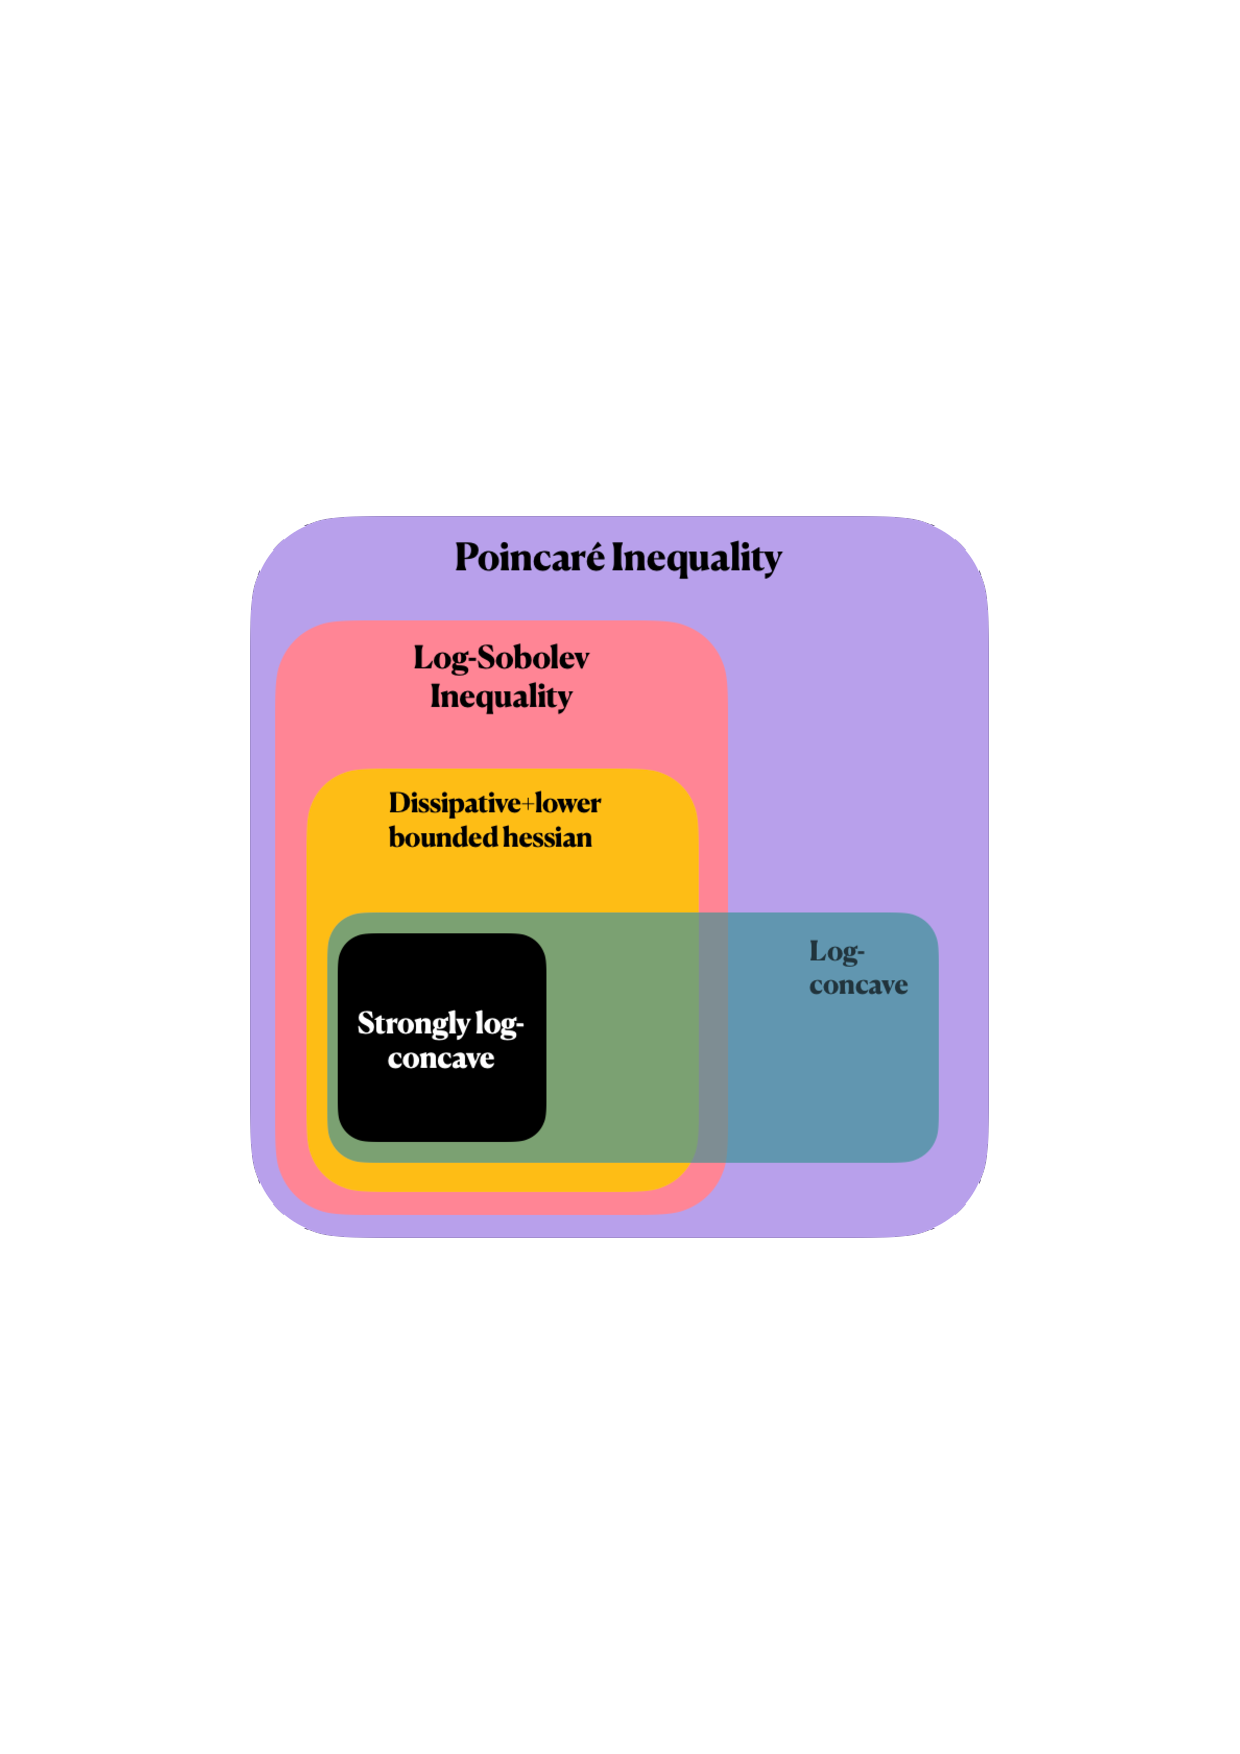
\includegraphics[width=0.5\textwidth]{diagram.pdf}
    \caption{A diagram showing the order between commonly used assumptions.  A proof that strongly-log concave densities are dissipative can be derived from the quadratic lower bound at $0$. Corollary 2.1.(2) of \cite{cattiaux_note_2010} shows that dissipativity and lower bounded hessians imply LSI. The fact that poincare inequalities  hold for log-concave measures is shown in Corollary 1.9 of \cite{bakry_simple_2008}. The proof that LSI implies Poincare can be found in \cite{bakry_markov_2014}(Proposition 5.1.3).}
    \label{fig:diagram}
\end{figure}

Is it only perturbations of strongly convex ?

Lipschitz mappings.

Implication of  quadratic growth might be restrictive so there are other inequalities that may be considered. 

Link with dissipativity. Is it stronger ? a better assumption, more used in optimization litterature. However, the other papers don't just use dissipativity to control, they use it to guarantee quadratic growth. And in particular they use it to bound the expected moments of the gradients.

This paper provides a proof of convergence in KL divergence of LMC under minimal assumptions of isoperimetry and smoothness.

The proof is based on considering the continuous time SDE of which 

\subsection{Conditional Fokker-Planck}

\subsection{Getting to Gronwall only using LSI and smoothness}

The first term in equation (*) can immediately be upperbounded using the LSI assumption. A central contribution of this paper is showing that 

\subsection{The Renyi Result}

The renyi results decompose into three parts. 
A considerably weaker result is provided for convergence of ULA measured in Renyi divergence.

Renyi, KL, Wassertein.
Discuss the different metrics and how different hypotheses on the warm start affect things.

\subsection{Discussion}

From theorem (*) it is possible to derive the number of iterations needed to be $\epsilon$-close in KL divergence to the target measure $\pi$. 

\section{Analyzing the trajectories of LMC}

To better understand how exponentially small LSI constants can affect the dynamics, we turn our attention to the work of Tzen, Liang and Raginsky \cite{tzen_local_2018}. 

The goal of their paper is to describe the behavior of the trajectories of LMC. Here, LMC is viewed as a tool to optimize the potential $f$. This introduces a parameter $\beta$, referred to as the \textit{inverse temperature} in our LMC iteration :
\begin{equation}
\label{eq:betaLMC}
\mathbf{X}_{k+1} = X_k - \eta \nabla f(X_k) + \sqrt{\frac{2\eta}{\beta}}Z_{k+1}
\tag{LMC-$\beta$}
\end{equation}
which is a discretization of the diffusion
\begin{equation}
\label{eq:betadiff}
\tag{LD-$\beta$}
dX_t = -\nabla f(X_t)dt + \sqrt{\frac{2}{\beta}}dB_t.
\end{equation}
The diffusion above has a stationary measure $\pi_\beta$ whose density is proportional to $e^{-\beta f}$. When $\beta \rightarrow \infty$, this stationary measure concentrates around the minimizers of $f$ (Section 3.5, \cite{raginsky_non-convex_2017}). Consequently, by choosing high enough values of $\beta$, we can optimize $f$ using \eqref{eq:betaLMC}.

Tzen et al study the behavior of the iterates of this algorithm around local minimizers of $f$ and they find that with an appropriate choice of $\eta$ and $\beta$, the iterates can be made to stay within the neighborhood of some local minimzer for an arbitrarely long time with high probability.

This indicates that the possibly slow mixing of LMC can be caused by the long times spent around local minimizers.


\subsection{Setting}

In \cite{tzen_local_2018}, the potential $f: \R^d \rightarrow \R$ on which LMC is applied is an empirical risk approximation of a population risk. Indeed, taking the population risk to be of the form
\(
F(x) : = \E_\nu [\ell(x, Z)]
\), where $Z \sim \nu$ is some unknown probability measure over some set $\mathcal{Z}$, we can attempt to optimize $F$ by considering the empirical risk
\begin{equation}
f(x) = \frac{1}{n} \sum_{i=1}^{n}\ell(x, Z_i),
\label{eq:ERM}
\end{equation}
where $Z_1, \dots, Z_n$ are independent, identically distributed samples from $\nu$. The following assumptions are made on the functions $\ell$ which translate to properties of $f$.
\begin{assumption}
  For any $z \in \mathcal{Z}$, the function $x \mapsto \ell(x, z)$ is continuously twice differentiable and there exists $B$ such that $\| \nabla \ell (0, z) \| \leq B$ for all $z \in \mathcal{Z}$.
\end{assumption}
\begin{assumption}
  There exist $L > 0$ and $M> 0$ such that for any $z \in \mathcal{Z}$,
  \[
  \| \nabla \ell(x, z) - \nabla \ell(y, z)\| \leq L \|x - y\| \quad \text{and} \quad \| \nabla^2 \ell(x, z) - \nabla^2 \ell(y, z)\|_2 \leq M \|x - y\|.
  \]
  This implies that $f$ is $L$-Lipschitz gradient and $M$-Lipschitz hessian.
\end{assumption}
\begin{assumption}
  The function $f$ is $(m, b)$-dissipative :
  \[
  \exists m>0, \; b\geq 0, \quad \forall x \in \R^d, \quad \langle x, \nabla f(x) \rangle \geq m \|w\|^2 - b.
  \]
\end{assumption}

We note in passing that these assumptions imply that $f$ verifies the LSI (see Figure \ref{fig:diagram}), but the problem of convergence to stationarity here is not considered here. Rather, Tzen et al focus on proving the following result on time spent around local minima when using \eqref{eq:betaLMC} to optimize \eqref{eq:ERM}.

\subsection{The main Result}

First, pick a nondegenerate local minimum $\bar{x}$ of $f$ where $H = \nabla^2f(\bar{x})$ is positive definite and initialize \eqref{eq:betaLMC} within a distance of at most $r > 0$ of $\bar{x}$. 

\begin{quote}
\begin{emph}
For any small $\epsilon >0$, we set $T_{rec} = \frac{2}{m} \log(\frac{8r}{\epsilon})$. For any escape time $T_{\text{esc}} > T_{\text{rec}}$ of our choice, there exist an $\eta$ small enough, scaling as $O(\frac{1}{T_{\text{esc}}})$, and a $\beta$ big enough, scaling as $O(\log(T_{\text{esc}}))$, such for the iterates of \eqref{eq:betaLMC} initialized at a distance at most $r$, we have
\[
\Prb(\text{Escape from neighborhood of $w_H$ in } [T_{\text{rec}}, T_{\text{esc}}]) \leq \delta.
\]
\end{emph}
\end{quote}

This result tells us that we can make the iterates of \eqref{eq:betaLMC} stay within the neighborhood of a local minimum for as long as we desire with an appropriate choice of $\eta$ and $\beta$.

\subsection{A summary of the proof}

We can briefly outline the main ideas underlying the proof.

The proof of this theorem proceeds as follows. First, the gradient is linearized around some local minimum. The behavior of the diffusion is the sum of two components : the easily controllable process, that we denote N for nice, coming, from the linear term and the bounded term coming from the inexact linearization. 

The goal is to control how the process deviates

The proof is an interesting strategy. First divide the process we want to control in two A and B with B being a process we can upper bound and A.

This way the burden of controlling the first term is entirely within my control because A is a martingale and there is a rich set of theorems controlling suprema of martingales.

Then stick together the result by using a union bound.

\subsection{Dealing with discretization}

Girsanov's theorem cite Oksendal which was used by Dalalyan for providing the first proof of LMC and RRT for the analysis of LMC with access to stochasitc estimates of $\nabla f$.

\subsection{Is this the theorem we were looking for ?}

In reading the theorem, we might take issue with the freedom we are given in setting the escape time $T_{\text{esc}}$. The theorem allows us to make  holds if we scale down the step size $\eta$ and scale up the parameter $\beta$ appropriately. In fact, this , the setting of the recurrence time seems to come out simply of analytic convenience, nothing in the proof 

\subsection{Kramers escape problem}

\section{LMC in the real world}

We have seen in the previous section that the price to pay for a small log-Sobolev constant is time exponentially long in the dimension spent around local minimizers. The question now is to figure out where real world distributions lie. Do they live in the untractable realm of exponentially small LSI constants ?

To try to answer this question, we study in this section the work of Song and Ermon \cite{song_generative_2019}. Their paper proposes a method for sampling from real world distributions by first learning the score from available data using a neural network then sampling from the learnt score using Langevin Monte Carlo. A naive application of this idea yields samples of poor quality and the authors show that, for this approach to work, the perturbation of the data by noise is instrumental.

We discuss their method in detail by first explaining how the score is learnt, then we describe the proposed LMC scheme and finish by arguing that the demonstrated success of \cite{song_generative_2019} provides strong support for the view that the real world is tractable.

\subsection{Score matching}

Score matching consists of learning the score of a distribution $\pi$ when only having access to independent samples.

A vector field $s_\theta: \R^d \rightarrow \R^d$ is parametrized with a neural network, where $\theta$ denotes the network parameters included in some set $\Theta$. This network is then trained to learn the score of the data distribution by minimizing the Fisher divergence 
\begin{equation}
\min_{\theta \in \Theta} \E_{X \sim \pi} \left[ \left\| \nabla \log p_\pi(X) - s_\theta(X) \right\|_2^2\right].
\label{eq:fisher}
\end{equation}
If the minimum $0$ is attained for some parameter $\theta^\star$, the equality $s_{\theta^\star} = \nabla \log p_\pi(x)$ will hold $\pi$-almost everywhere. The loss \eqref{eq:fisher} is therefore a sensible one. But since it involves the unknown score $\nabla \log p_\pi(x)$, it is unusable in practice.

Hyv\"arinen \cite{hyvarinen_estimation_2005} noticed that if $p_\pi$ is decays sufficiently fast at infinity, such that for any $\theta \in \Theta$,
\(
 \lim_{\|x\|_2 \rightarrow \infty} p(x)s_\theta(x) =0,
\)
then, a simple integration by parts will to the equivalent optimization problem
\begin{equation}
\min_{\theta \in \Theta} \E_{X \sim \pi} \left[ \text{tr}(J_{s_\theta}(X)) + \|s_\theta(X)\|_2^2\right],
\label{eq:tractable-score}
\end{equation}
where $J_{s_\theta}(x)$ denotes the Jacobian of $s_\theta$ at $x$. Although this is now implementable, the trace of the Jacobian is an expensive quantity to compute. Two methods to alleviate this computational burden are discussed in \cite{song_generative_2019}.

The first is \textit{sliced score matching}, proposed by Song and his collaborators, replaces the trace by an unbiased estimator $v^TJ{s_\theta}(X)v$ where $v$ is an isotropic random vector, in order to leverage the fast implementation of Jacobian-vector products available in automatic differentiation packages. The second method, better suited for the scores involved in this paper, is \textit{Denoising Score Matching (DSM)} \cite{vincent_connection_2011}. Unlike sliced score matching, DSM does not estimate the score of the data distribution $\pi$ but rather the score of data distribution perturbed by Gaussian noise $p * \mathcal{N}(0, \sigma^2I)$. An integration by parts shows that learning scores of perturbed distributions amounts to minimizing the implementable loss
\[
\min_{\theta \in \Theta} \E_{X \sim \pi, Z \sim \mathcal{N}(0, \sigma^2I)} \left[ \|s_\theta(X + Z) -  \frac{Z}{2\sigma^2}\|_2^2\right].
\]

Learning the perturbed score is well suited here because, as we will see next, perturbation is necessary for score matching to work well.

\subsection{The need for noise}
\label{sec:noise}

Given a set of samples from some real world distribution, attempting to minimize \eqref{eq:tractable-score} is likely to fail.

First, \eqref{eq:tractable-score} assumes that a score exists. This requires that the data distribution admit a density with respect to the Lebesgue measure that is differentiable and positive over the entire space. There is no reason to believe this is the case for the distribution of natural images. In fact, a commonly held belief is that the support of this natural distribution is some lower dimensional manifold to which the Lebesgue measure assigns no mass. Therefore, it is unrealistic to expect that this distribution admits density let alone a differentiable one.

Moreover, the loss in \eqref{eq:tractable-score} is a weighted $L_2$ loss that enforces score matching in regions of high probability and discounts mismatches in low probability regions. This causes the learnt score to be innacurate in low probability regions. The aim being to apply a random walk algorithm that traverses the space, going from one high probability region to another, low accuracy score matching are likely to induce it in error. 

Gaussian smoothing can address both these issues. Indeed, convolution by a Gaussian confers all the necessary regularity : first, convolution with a absolutely continuous distribution like the Gaussian guarantees the existence of a density with respect to the Lebesgue measure, second, since the Gaussian is infinitely supported, the density is positive everywhere, and finally the continuous differentiability of the Gaussian density is inherited by the density. Moreover, perturbation with a Gaussian with high enough variance increases the likelihood that samples will land in regions that were originally of low probability. This improves the score matching in those regions.

The addition of noise to the samples is therefore crucial to successfully match the score of the data distribution. It ensures the well-posedness of the problem and improves the matching in low data density regions.

\subsection{Learning the score in practice}

Inspired by simulated annealing, the authors propose to perturb the data with a decreasing sequence of noise scales and learning, jointly, the scores of the decreasingly perturbed distributions. The proposed method consists of first setting a geometrically decreasing sequence of noise scales $\sigma_1 > \dots > \sigma_L$. A \textif{conditional}\footnote{Here, conditional is borrowed from the deep learning litterature, and simply means that the input variable is augmented with an additional input to \textit{condition} the output.} neural network $s_\theta(x, \sigma)$, referred to as a \textit{Noise Conditional Score Network}, is chosen to parametrize the $L$  vector fields that will be matched to the gradient fields associated to each of the perturbed distribution.

For each of the noise scales, the loss defined in \eqref{eq:tractable-score} is denoted $\ell(\theta, \sigma)$. The network is then trained to jointly minimize all those losses by enforcing the minimization of
\[
\frac{1}{L} \sum_{i=1}^{L}\lambda(\sigma_i) \ell(\theta, \sigma_i),
\]
where $\lambda(\sigma_i)$ is a weighing coefficient set to $\sigma_i^2$ to ensure that the products \(\lambda(\sigma_i) \ell(\theta, \sigma_i)\) are roughly of the same order for each noise scale $\sigma_i$. 

To learn the score of an image distribution, the authors recommend using an architecture that is well suited for image classification. In the experiments, a U-Net architecture is chosen to parametrize the vector fields, it is trained with Adam.


\subsection{Annealed Langevin Dynamics}

Once the score network trained, the next step is now to sample from the distribution it represents using LMC. Although our ultimate goal is to sample from the data distribution, we know, from the discussion in \ref{sec:noise}, that the best we can do is to sample from the least perturbed distribution.

Following the simulated annealing inspiration, the authors propose that instead of directly attempting to sample from the least perturbed distribution, it is better to use the sequence of scores to progressively warm start LMC at each round. The algorithm proceeds as follows : an initial sample is drawn form a uniform distribution over the hypercube, then LMC is run for T steps to sample from $\pi_{\sigma_0}$, the output is then used to as the initial point for sampling from the next noise level. The pseudo-code is provided in \ref{alg:anneal}.

\begin{algorithm}
	\caption{Annealed Langevin dynamics.}
	\label{alg:anneal}
	\begin{algorithmic}[1]
	    \REQUIRE{$\{\sigma_i\}_{i=1}^L, \eta, T$.}
	    \STATE{Initialize $\tilde{\bfx}_0$}
	    \FOR{$i \gets 1$ to $L$}
	        \STATE{$\eta_i \gets \eta \cdot \sigma_i^2/\sigma_L^2$} \Comment{$\eta_i$ is the step size for noise level $\sigma_i$}
            \FOR{$t \gets 1$ to $T$}
                \STATE{Draw $z_t \sim \mathcal{N}(0, I)$}
                \STATE{{$\tilde{\bfx}_{t} \gets \tilde{\bfx}_{t-1} + \eta_i s_\theta(\tilde{\bfx}_{t-1}, \sigma_i) + \sqrt{2\eta_i}~ z_t$}}
            \ENDFOR
            \STATE{$\tilde{\bfx}_0 \gets \tilde{\bfx}_T$}
        \ENDFOR
        \STATE{ \Return $\tilde{\bfx}_T$}
	\end{algorithmic}
\end{algorithm}

What is suprising here are the chosen hyperparameters. The results were obtained with very few iterations of LMC for each noise level. The time T is kept constant for each noise level and the reported images were obtained for $T=100$, a very small value in view of the dimension dependence we expect from our convergence bounds.
\subsection{Evaluation metrics}

The small value of $T$ is only notable if the method is successful. We discuss the two metrics reported in the paper : the Inception score and the FID score. We briefly describe them to understand the properties they are evaluating.

\paragraph{Inception score} For a given generative model $G$, we write $X \sim G$, for the samples generated by $G$. We define the class distribution $\Prb_Y := \texttt{Inceptionv3(X)}$, where \texttt{Inceptionv3} is a convolutional neural network trained for classification on the same dataset $G$ was trained on. It outputs a distribution over the class labels. The Inception score IS$(G)$ is then defined as 
\[
\text{IS}(G) = \exp \left(\E_{X \sim G} [KL(\Prb_{Y|X} || \Prb_Y)] \right).
\]

\paragraph{FID score}  An improvement over the Inception score was proposed by \cite{heusel_gans_2017}. The \textit{Frechet Inception Distance}(FID) also makes use of a trained \texttt{Inceptionv3}. Two statistics, the mean and the variance, of the intermediate features extracted by the network are computed. These two quantities are then used to define a Gaussian random variable. The FID score is taken to be the Wassertein distance between this Gaussian and the one obtained from real data.

In addition to these quantitative metrics, the authors provide uncurated images that they have sampled using their method. The images look compelling, although this remains a subjective judgment. A nearest neighbor analysis of a few samples, which consists of looking for the closest image in $\ell_2$ norm in the training dataset, reveals that the samples are not merely memorized. 

According to these measures of success, it is reasonable to state that the NCNS + Annealed Langevin scheme is succesful in sampling from real image distributions.

\subsection{Discussion}

The least convincing part of the paper is the discussion in Section 3.2.2. There it is argued that since LMC is blind to the mixing coefficients it will struggle with sampling from mixtures. We know from our previous study of LMC that this is not the cause for the difficulty of sampling, it is merely because jumping from one mode to the other takes time when the modes are well separated.

Other than this minor point, the paper does a great job at showing that LMC can be succesful is sampling from real world distributions. Many of the unjustified or hand-wavy arguments in the paper for choosing the constants are reevaluated and given more precision in a follow-up paper. Currently, approaches that share strong similarities with this one are the best at sampling from a wide array of image datasets.

\section{Conclusion and open questions}

Niles Weed result.
SGD; adaptively preconditionned methods; dangers of SGD

What about saddle points ? A convergence bound involving weaker assumptions will allow us to prove the polynomial time escape from saddle points of perturbed gradient descent.

Tools to analyze recurrences involving gradients and noise which is of high interest in machine learning.

There are currently not many works studying adaptively preconditionned methods. 


\bibliography{references.bib}


% Computer Society journal papers do something a tad strange with the very
% first section heading (almost always called "Introduction"). They place it
% ABOVE the main text! IEEEtran.cls currently does not do this for you.
% However, You can achieve this effect by making LaTeX jump through some
% hoops via something like:
%
%\ifCLASSOPTIONcompsoc
%  \noindent\raisebox{2\baselineskip}[0pt][0pt]%
%  {\parbox{\columnwidth}{\section{Introduction}\label{sec:introduction}%
%  \global\everypar=\everypar}}%
%  \vspace{-1\baselineskip}\vspace{-\parskip}\par
%\else
%  \section{Introduction}\label{sec:introduction}\par
%\fi
%
% Admittedly, this is a hack and may well be fragile, but seems to do the
% trick for me. Note the need to keep any \label that may be used right
% after \section in the above as the hack puts \section within a raised box.



% The very first letter is a 2 line initial drop letter followed
% by the rest of the first word in caps (small caps for compsoc).
% 
% form to use if the first word consists of a single letter:
% \IEEEPARstart{A}{demo} file is ....
% 
% form to use if you need the single drop letter followed by
% normal text (unknown if ever used by IEEE):
% \IEEEPARstart{A}{}demo file is ....
% 
% Some journals put the first two words in caps:
% \IEEEPARstart{T}{his demo} file is ....
% 
% Here we have the typical use of a "T" for an initial drop letter
% and "HIS" in caps to complete the first word.
\IEEEPARstart{T}{his} template is not trying to suggest a specific
style for the content of your candidacy exam/thesis proposal paper; it
only concerns the style of the writeup itself.  This template is in LaTeX.
We encourage you to use it for your write-up.

If you insist on using a different word processing program please
match the style as much as possible.  Here is the basic format: The
paper size is A4, the font is 10 point, 
single-spacing, ``times roman like.''
Two columns, each 8.75~cm wide, with 1.5~cm left/right margins.
Sections and sub-sections have bold numbered headings.  Figures have
captions underneath, with a bold label and number, and also a short
caption sentence.  Ditto for tables.  The text itself is a mix of standard
paragraphs, bullets, numbered lists, and equations where appropriate.
References are at the end, in a numbered format, in a slightly smaller
font.

The overall length of this write-up should be 4-8 pages. 

\subsection{Purpose of this Write-Up}
% needed in second column of first page if using \IEEEpubid
%\IEEEpubidadjcol
This write-up serves two purposes. First, it forms the basis for
your candidacy exam. As such you should summarize the three papers selected
by your advisor and yourself, and analyze as well as discuss them critically.
Second, the write-up 
is also your thesis proposal.  Therefore, the last one or two pages should
be dedicated to your own preliminary work. A road-map of how you plan to
advance the state of the art in your chosen area should also be given.
For further details please consult the document ``PhD Candidacy Exam Overview.'' You can find the latest
version at {\tt http://phd.epfl.ch/page57746-en.html}.


\subsection{What to Put into the Introduction}
Describe briefly the context, the problem, shortcomings in prior
approaches, and your proposed approach and solution. Forecast results.


% An example of a floating figure using the graphicx package.
% Note that \label must occur AFTER (or within) \caption.
% For figures, \caption should occur after the \includegraphics.
% Note that IEEEtran v1.7 and later has special internal code that
% is designed to preserve the operation of \label within \caption
% even when the captionsoff option is in effect. However, because
% of issues like this, it may be the safest practice to put all your
% \label just after \caption rather than within \caption{}.
%
% Reminder: the "draftcls" or "draftclsnofoot", not "draft", class
% option should be used if it is desired that the figures are to be
% displayed while in draft mode.
%
%\begin{figure}[!t]
%\centering
%\includegraphics[width=2.5in]{myfigure}
% where an .eps filename suffix will be assumed under latex, 
% and a .pdf suffix will be assumed for pdflatex; or what has been declared
% via \DeclareGraphicsExtensions.
%\caption{Simulation Results}
%\label{fig_sim}
%\end{figure}

% Note that IEEE typically puts floats only at the top, even when this
% results in a large percentage of a column being occupied by floats.
% However, the Computer Society has been known to put floats at the bottom.


% An example of a double column floating figure using two subfigures.
% (The subfig.sty package must be loaded for this to work.)
% The subfigure \label commands are set within each subfloat command, the
% \label for the overall figure must come after \caption.
% \hfil must be used as a separator to get equal spacing.
% The subfigure.sty package works much the same way, except \subfigure is
% used instead of \subfloat.
%
%\begin{figure*}[!t]
%\centerline{\subfloat[Case I]\includegraphics[width=2.5in]{subfigcase1}%
%\label{fig_first_case}}
%\hfil
%\subfloat[Case II]{\includegraphics[width=2.5in]{subfigcase2}%
%\label{fig_second_case}}}
%\caption{Simulation results}
%\label{fig_sim}
%\end{figure*}
%
% Note that often IEEE papers with subfigures do not employ subfigure
% captions (using the optional argument to \subfloat), but instead will
% reference/describe all of them (a), (b), etc., within the main caption.


% An example of a floating table. Note that, for IEEE style tables, the 
% \caption command should come BEFORE the table. Table text will default to
% \footnotesize as IEEE normally uses this smaller font for tables.
% The \label must come after \caption as always.
%
%\begin{table}[!t]
%% increase table row spacing, adjust to taste
%\renewcommand{\arraystretch}{1.3}
% if using array.sty, it might be a good idea to tweak the value of
% \extrarowheight as needed to properly center the text within the cells
%\caption{An Example of a Table}
%\label{table_example}
%\centering
%% Some packages, such as MDW tools, offer better commands for making tables
%% than the plain LaTeX2e tabular which is used here.
%\begin{tabular}{|c||c|}
%\hline
%One & Two\\
%\hline
%Three & Four\\
%\hline
%\end{tabular}
%\end{table}






% if have a single appendix:
%\appendix[Proof of the Zonklar Equations]
% or
%\appendix  % for no appendix heading
% do not use \section anymore after \appendix, only \section*
% is possibly needed

% use appendices with more than one appendix
% then use \section to start each appendix
% you must declare a \section before using any
% \subsection or using \label (\appendices by itself
% starts a section numbered zero.)
%


%\appendices
%\section{Proof of the First Zonklar Equation}
%Appendix one text goes here.

% you can choose not to have a title for an appendix
% if you want by leaving the argument blank
%\section{}

% use section* for acknowledgement
%\ifCLASSOPTIONcompsoc
%  % The Computer Society usually uses the plural form
%  \section*{Acknowledgments}
%\else
%  % regular IEEE prefers the singular form
%  \section*{Acknowledgment}
%\fi
%
%
%The authors would like to thank...
%
%
% Can use something like this to put references on a page
% by themselves when using endfloat and the captionsoff option.
%\ifCLASSOPTIONcaptionsoff
%  \newpage
%\fi



% trigger a \newpage just before the given reference
% number - used to balance the columns on the last page
% adjust value as needed - may need to be readjusted if
% the document is modified later
%\IEEEtriggeratref{8}
% The "triggered" command can be changed if desired:
%\IEEEtriggercmd{\enlargethispage{-5in}}

% references section

% can use a bibliography generated by BibTeX as a .bbl file
% BibTeX documentation can be easily obtained at:
% http://www.ctan.org/tex-archive/biblio/bibtex/contrib/doc/
% The IEEEtran BibTeX style support page is at:
% http://www.michaelshell.org/tex/ieeetran/bibtex/
%\bibliographystyle{IEEEtran}
% argument is your BibTeX string definitions and bibliography database(s)
%\bibliography{IEEEabrv,../bib/paper}
%
% <OR> manually copy in the resultant .bbl file
% set second argument of \begin to the number of references
% (used to reserve space for the reference number labels box)
\begin{thebibliography}{1}

\bibitem{mittelbach}
F.~Mittelbach, M.~Goossens, J.~Braams, D.~Carlisle, and C.~Rowley, 
\emph{The {\LaTeX}} Companion, 2nd~ed.\hskip 1em plus
0.5em minus 0.4em\relax Addison-Wesley Professional, 2004.

\end{thebibliography}

% biography section
% 
% If you have an EPS/PDF photo (graphicx package needed) extra braces are
% needed around the contents of the optional argument to biography to prevent
% the LaTeX parser from getting confused when it sees the complicated
% \includegraphics command within an optional argument. (You could create
% your own custom macro containing the \includegraphics command to make things
% simpler here.)
%\begin{biography}[{\includegraphics[width=1in,height=1.25in,clip,keepaspectratio]{mshell}}]{Michael Shell}
% or if you just want to reserve a space for a photo:

%\begin{IEEEbiography}{Michael Shell}
%Biography text here.
%\end{IEEEbiography}

% if you will not have a photo at all:
%\begin{IEEEbiographynophoto}{John Doe}
%Biography text here.
%\end{IEEEbiographynophoto}

% insert where needed to balance the two columns on the last page with
% biographies
%\newpage

%\begin{IEEEbiographynophoto}{Jane Doe}
%Biography text here.
%\end{IEEEbiographynophoto}

% You can push biographies down or up by placing
% a \vfill before or after them. The appropriate
% use of \vfill depends on what kind of text is
% on the last page and whether or not the columns
% are being equalized.

%\vfill

% Can be used to pull up biographies so that the bottom of the last one
% is flush with the other column.
%\enlargethispage{-5in}



% that's all folks
\end{document}


